% Hình bổ sung
\chapter{Hình bổ sung về telemetry và observability}

Phụ lục này tập hợp các ảnh Grafana/Prometheus và Hubble bổ sung cho phần phân tích ở Chương 4. Các ảnh trong phụ lục không phải là kết quả benchmark chính và không thay thế các biểu đồ p99, RPS, delta hoặc bảng thống kê. Vai trò của chúng là cung cấp thêm bối cảnh vận hành, hỗ trợ kiểm tra rằng các kết luận chính không bị chi phối bởi một dấu hiệu resource saturation hiển nhiên, đồng thời minh họa khả năng quan sát flow/verdict bằng Hubble trong Mode B.

Khi đọc các hình trong phụ lục, cần lưu ý rằng ảnh dashboard là snapshot theo cửa sổ thời gian, không phải time series đã được căn chỉnh chính xác với từng Fortio run hoặc từng pha trong S2. Vì vậy, chúng chỉ nên được dùng như bằng chứng hỗ trợ/sanity check, không dùng để kết luận định lượng về mức tiêu thụ CPU/memory của từng mode.

\section{Ảnh Grafana tổng quan}

Các ảnh tổng quan dưới đây minh họa các nhóm panel được dùng khi quan sát CPU, memory và network trong quá trình benchmark. Đây là cơ sở để đối chiếu bối cảnh vận hành, nhưng không phải nguồn chính để tính p99, RPS hoặc ý nghĩa thống kê.

\begin{figure}[H]
    \centering
    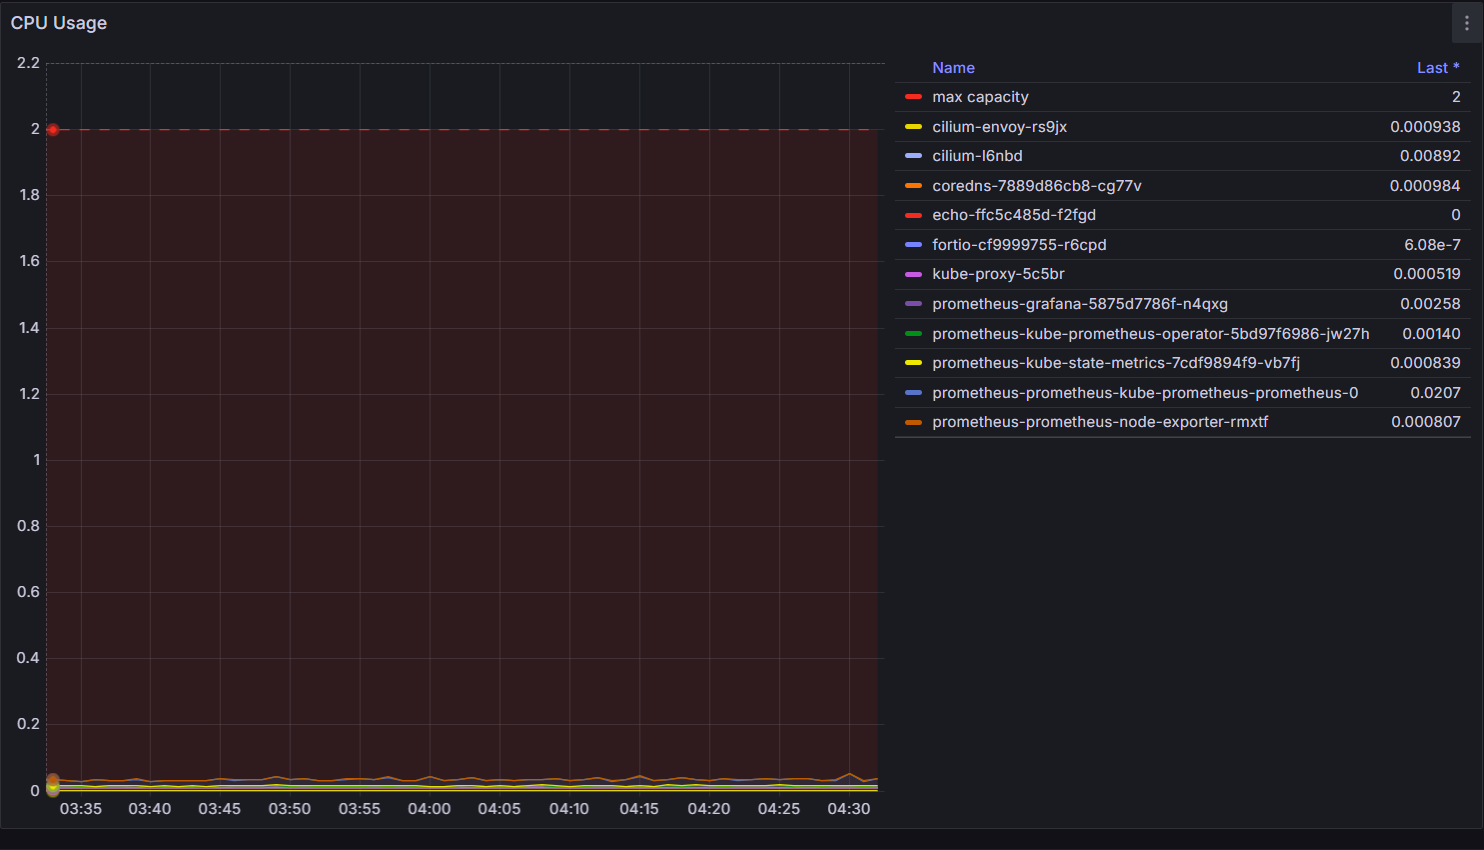
\includegraphics[width=0.92\textwidth]{../figures/grafana/fig-G1-grafana-cpu-node-pod.png}
    \caption{Panel Grafana/Prometheus tổng quan về CPU theo node/pod}
    \label{fig:app-grafana-cpu-node-pod}
\end{figure}

\begin{figure}[H]
    \centering
    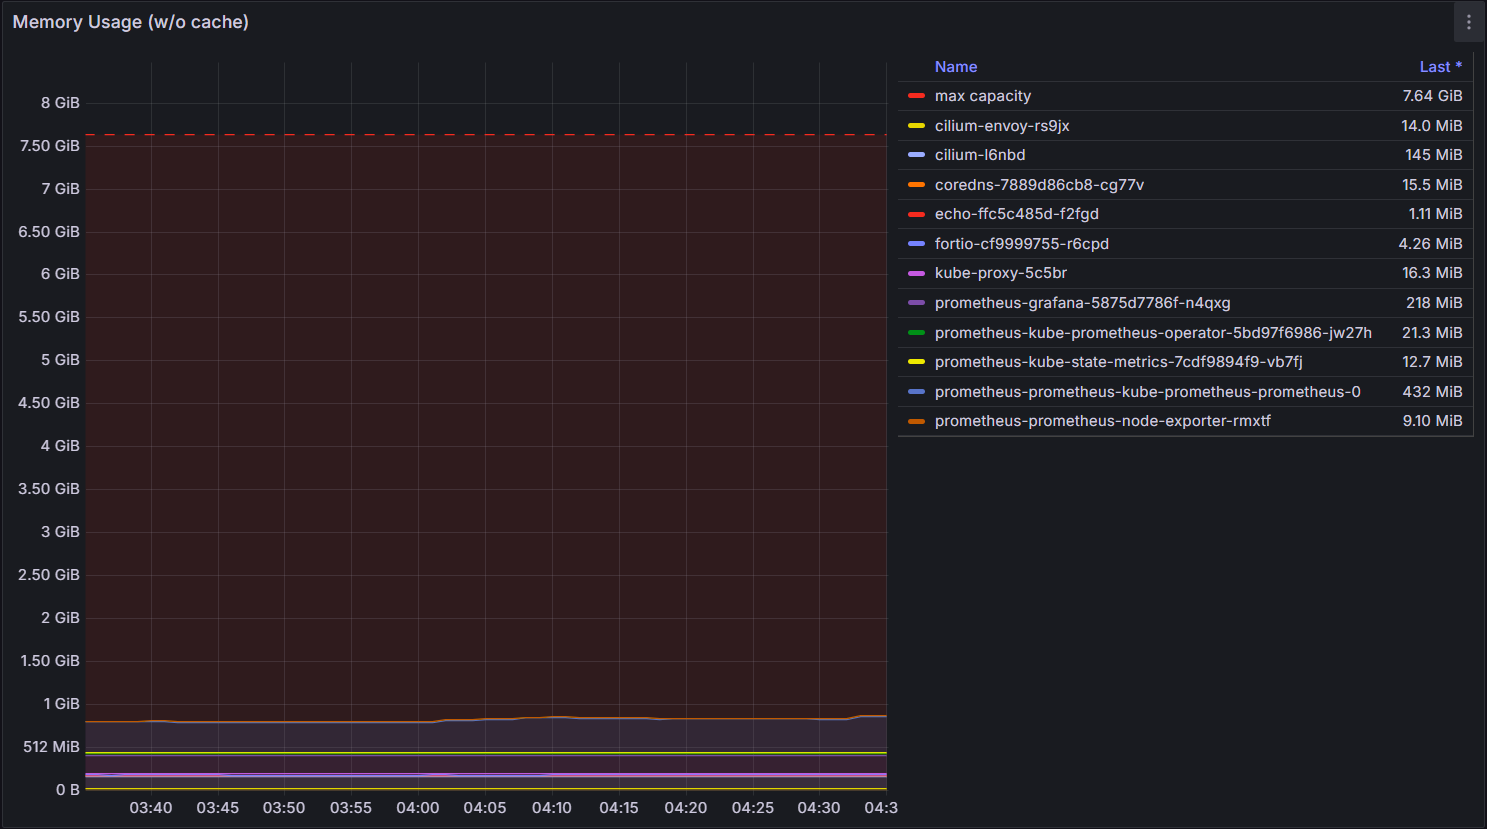
\includegraphics[width=0.92\textwidth]{../figures/grafana/fig-G3-grafana-memory-node-pod.png}
    \caption{Panel Grafana/Prometheus tổng quan về memory theo node/pod}
    \label{fig:app-grafana-memory-node-pod}
\end{figure}

\begin{figure}[H]
    \centering
    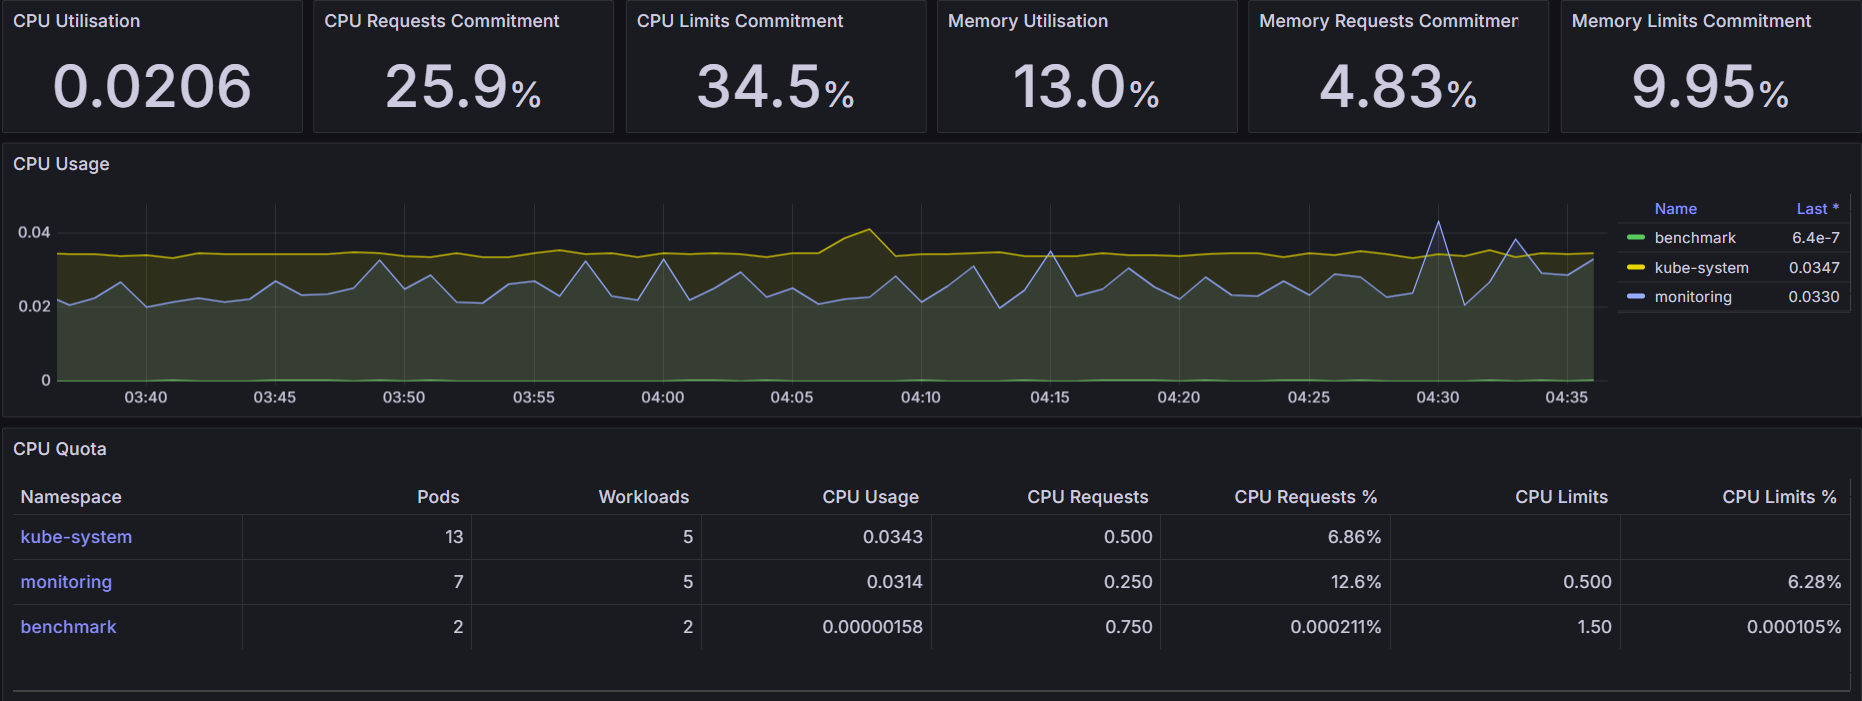
\includegraphics[width=0.92\textwidth]{../figures/grafana/fig-G4-grafana-cluster-overview.png}
    \caption{Panel Grafana/Prometheus tổng quan về trạng thái cluster}
    \label{fig:app-grafana-cluster-overview}
\end{figure}

\begin{figure}[H]
    \centering
    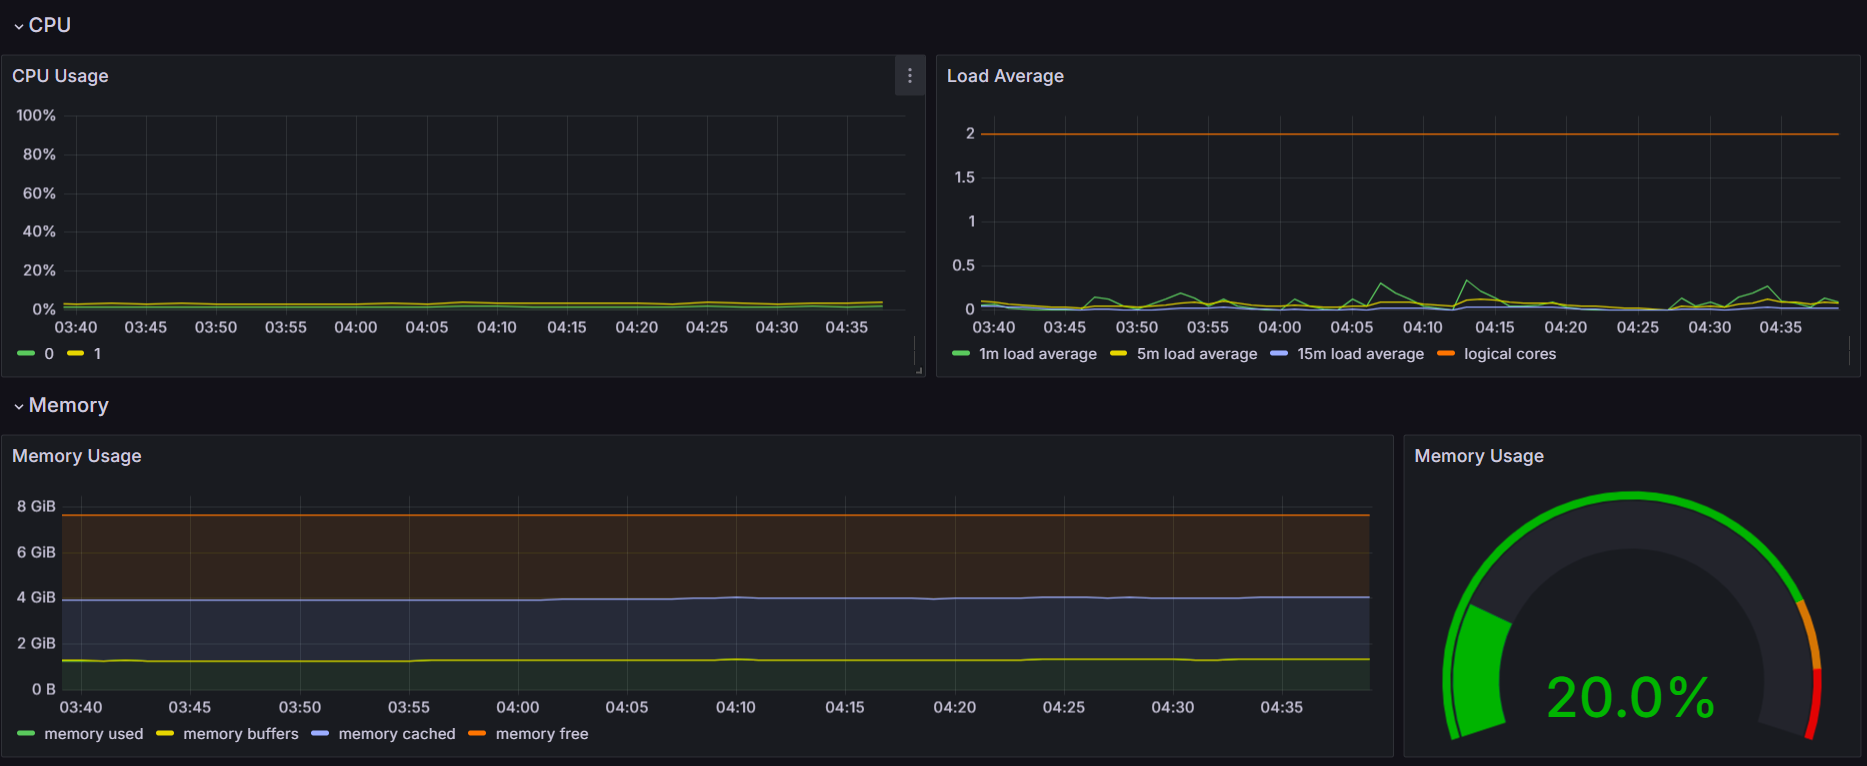
\includegraphics[width=0.92\textwidth]{../figures/grafana/fig-G5-grafana-node-network.png}
    \caption{Panel Grafana/Prometheus tổng quan về network theo node}
    \label{fig:app-grafana-node-network}
\end{figure}

\section{Ảnh Grafana bổ sung cho S1}

Các ảnh S1 L2 giúp kiểm tra bối cảnh CPU/memory ở mức namespace cho cả hai mode. Ảnh chính trong Chương 4 tập trung vào S1 L3 vì đó là mức tải có chênh lệch p99 rõ hơn; các ảnh dưới đây chỉ đóng vai trò bổ sung.

\begin{figure}[H]
    \centering
    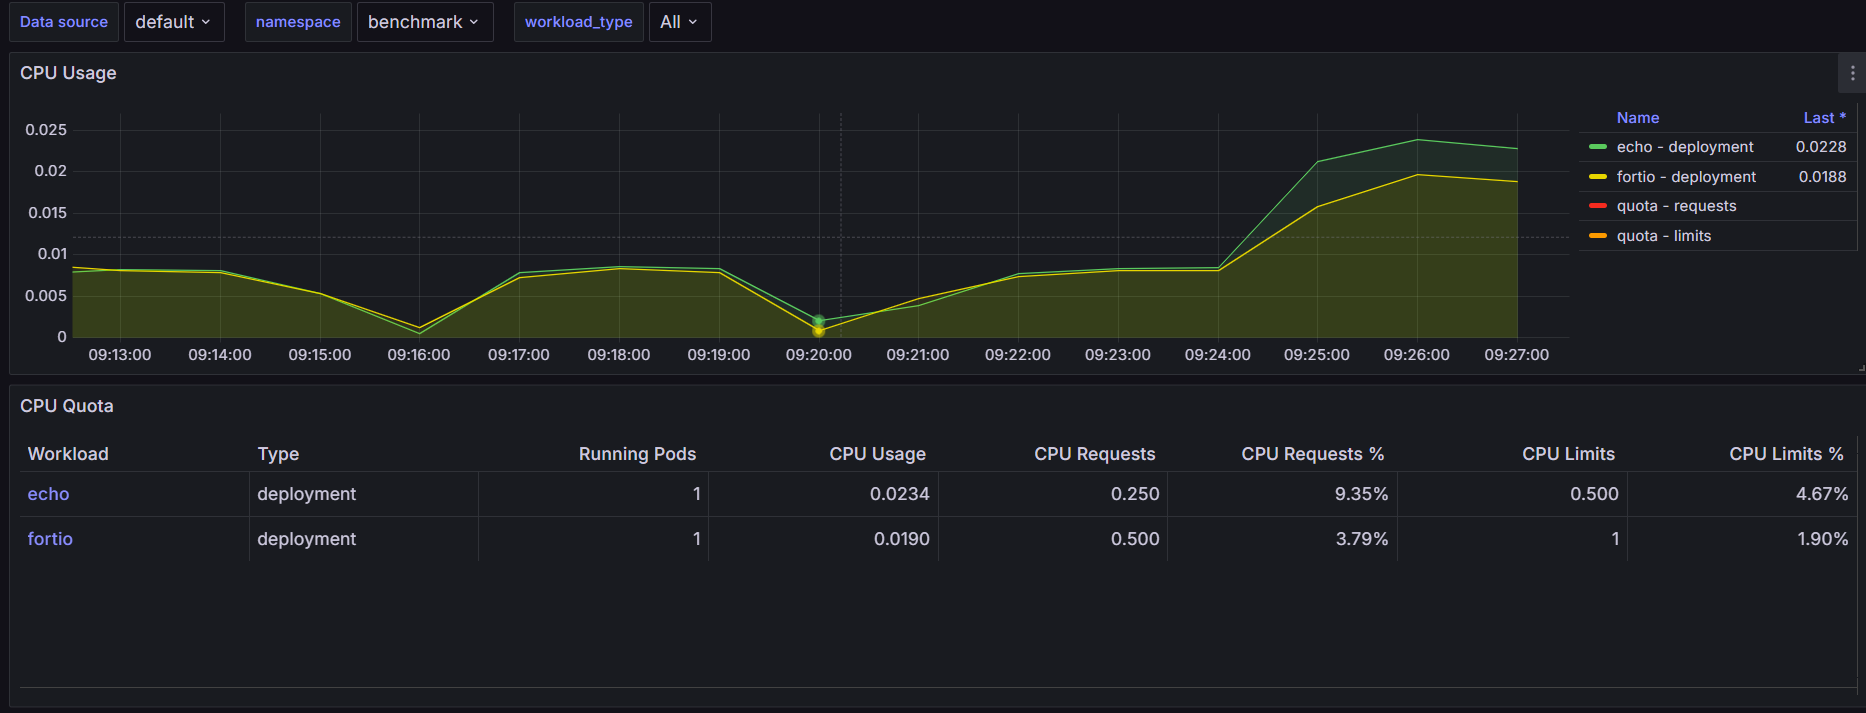
\includegraphics[width=0.92\textwidth]{../figures/grafana/modeA/grafana-ns-cpu-S1-L2-R1.png}
    \caption{Grafana bổ sung cho S1 L2 Mode A: CPU namespace}
    \label{fig:app-s1-l2-modea-cpu}
\end{figure}

\begin{figure}[H]
    \centering
    
\includegraphics[width=0.92\textwidth]{../figures/grafana/modeB/grafana-ns-cpu-S1-L2-R1.png}
    \caption{Grafana bổ sung cho S1 L2 Mode B: CPU namespace}
    \label{fig:app-s1-l2-modeb-cpu}
\end{figure}

\begin{figure}[H]
    \centering
    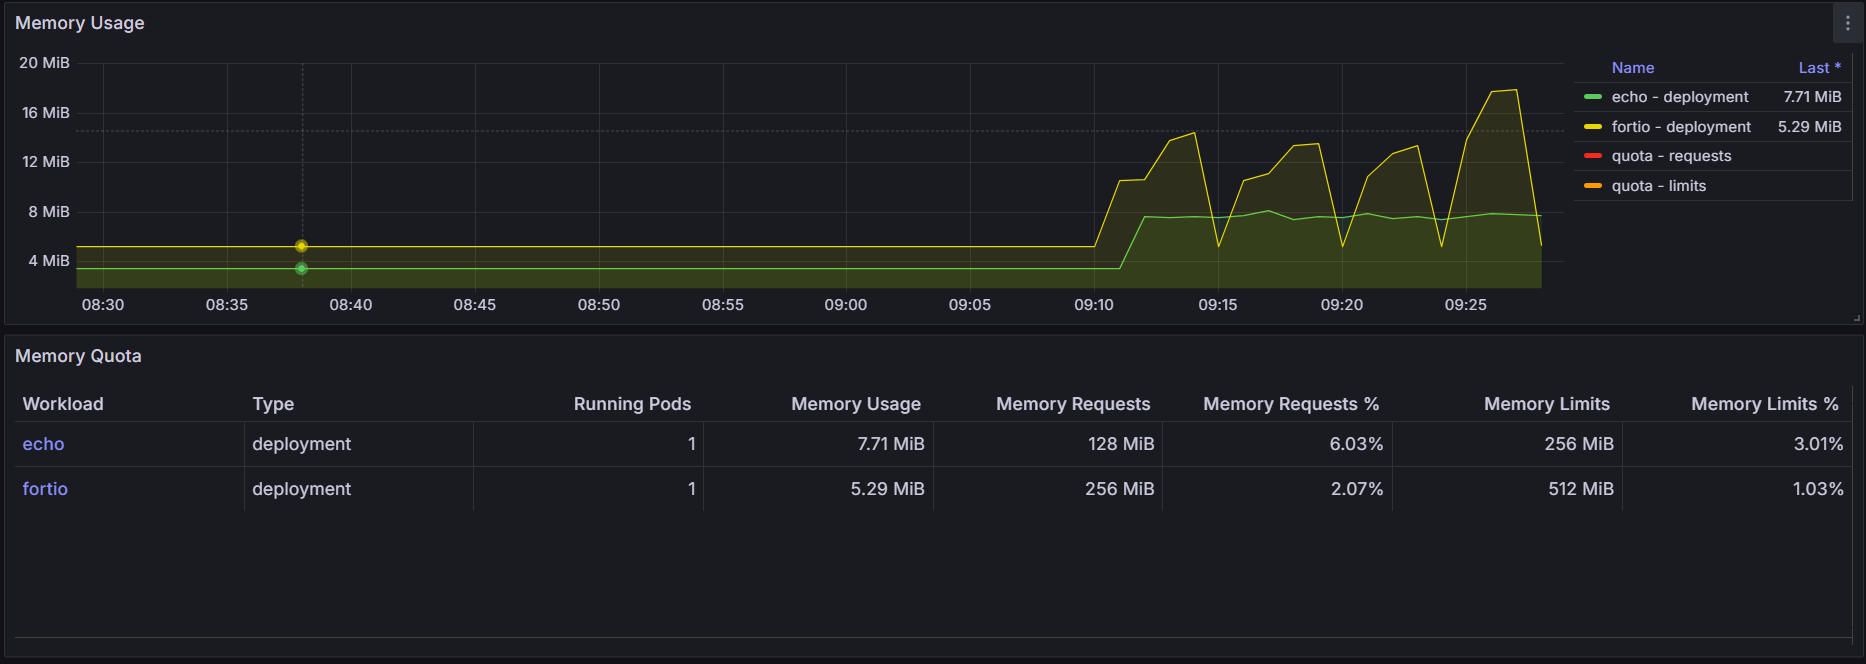
\includegraphics[width=0.92\textwidth]{../figures/grafana/modeA/grafana-ns-mem-S1-L2-R1.png}
    \caption{Grafana bổ sung cho S1 L2 Mode A: memory namespace}
    \label{fig:app-s1-l2-modea-memory}
\end{figure}

\begin{figure}[H]
    \centering
    
\includegraphics[width=0.92\textwidth]{../figures/grafana/modeB/grafana-ns-mem-S1-L2-R1.png}
    \caption{Grafana bổ sung cho S1 L2 Mode B: memory namespace}
    \label{fig:app-s1-l2-modeb-memory}
\end{figure}

\section{Ảnh Grafana bổ sung cho S2}

Các ảnh S2 L2 hỗ trợ đọc caveat của S2: biến động theo pha và churn cần được diễn giải thận trọng, thay vì quy trực tiếp cho resource pressure từ một ảnh dashboard.

\begin{figure}[H]
    \centering
    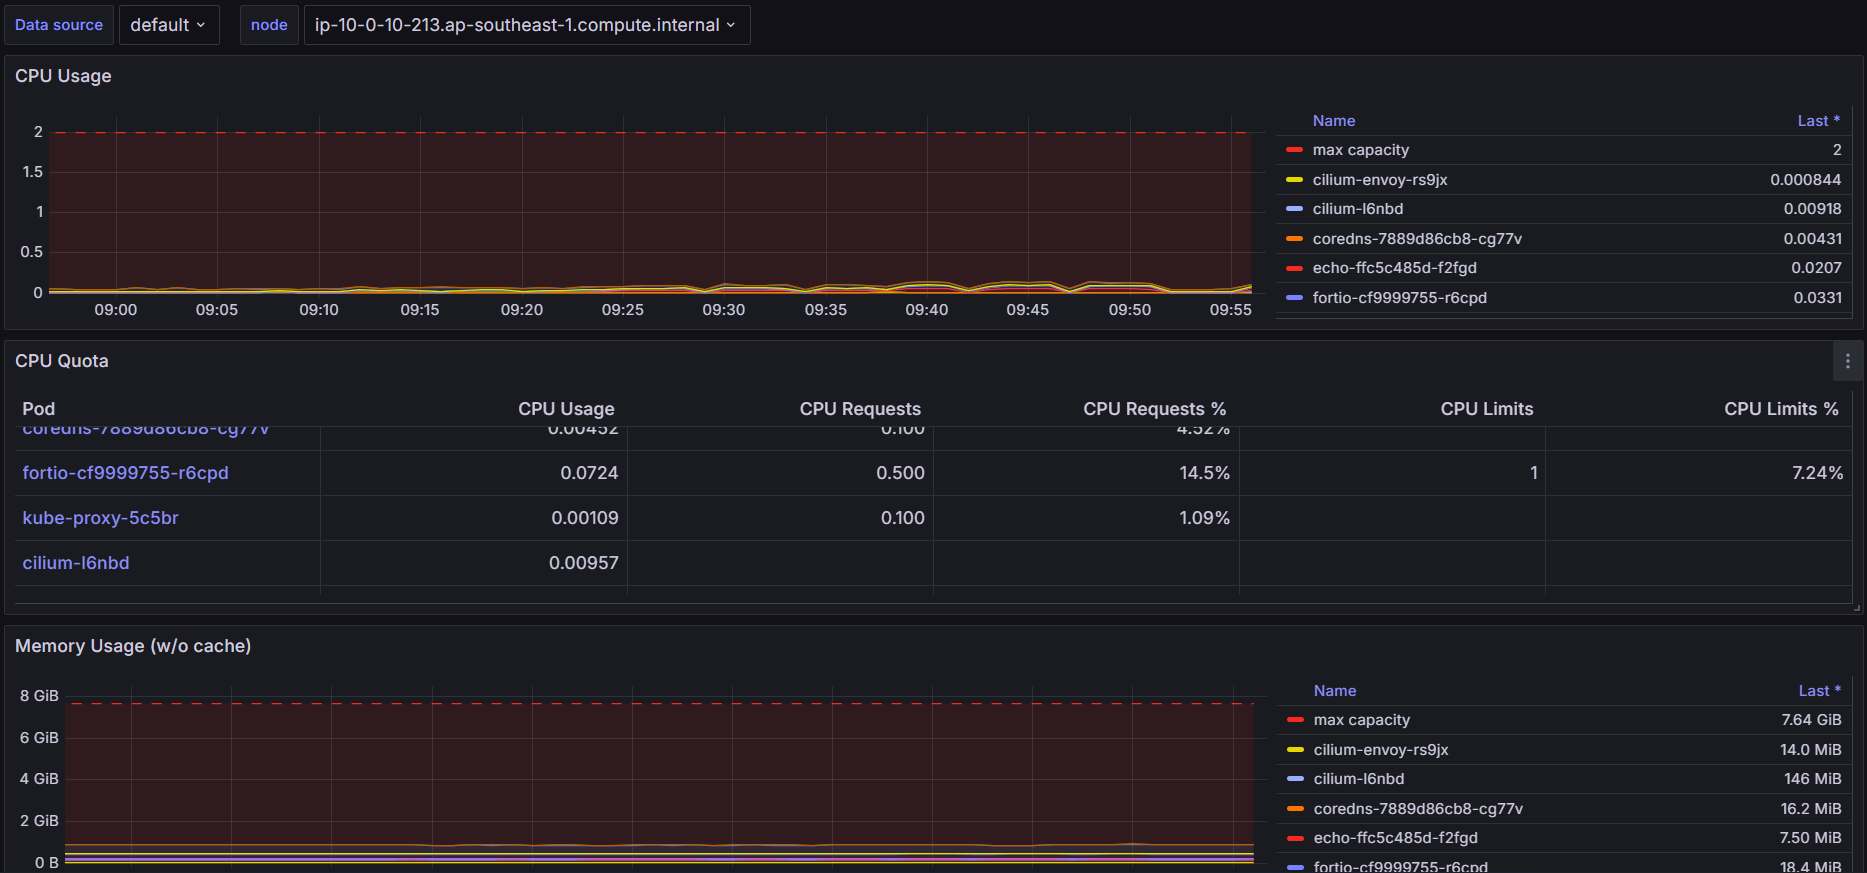
\includegraphics[width=0.92\textwidth]{../figures/grafana/modeA/grafana-node-cpu-mem-S2-L2-R1.png}
    \caption{Grafana bổ sung cho S2 L2 Mode A: node CPU/memory}
    \label{fig:app-s2-l2-modea-node-cpu-memory}
\end{figure}

\begin{figure}[H]
    \centering
    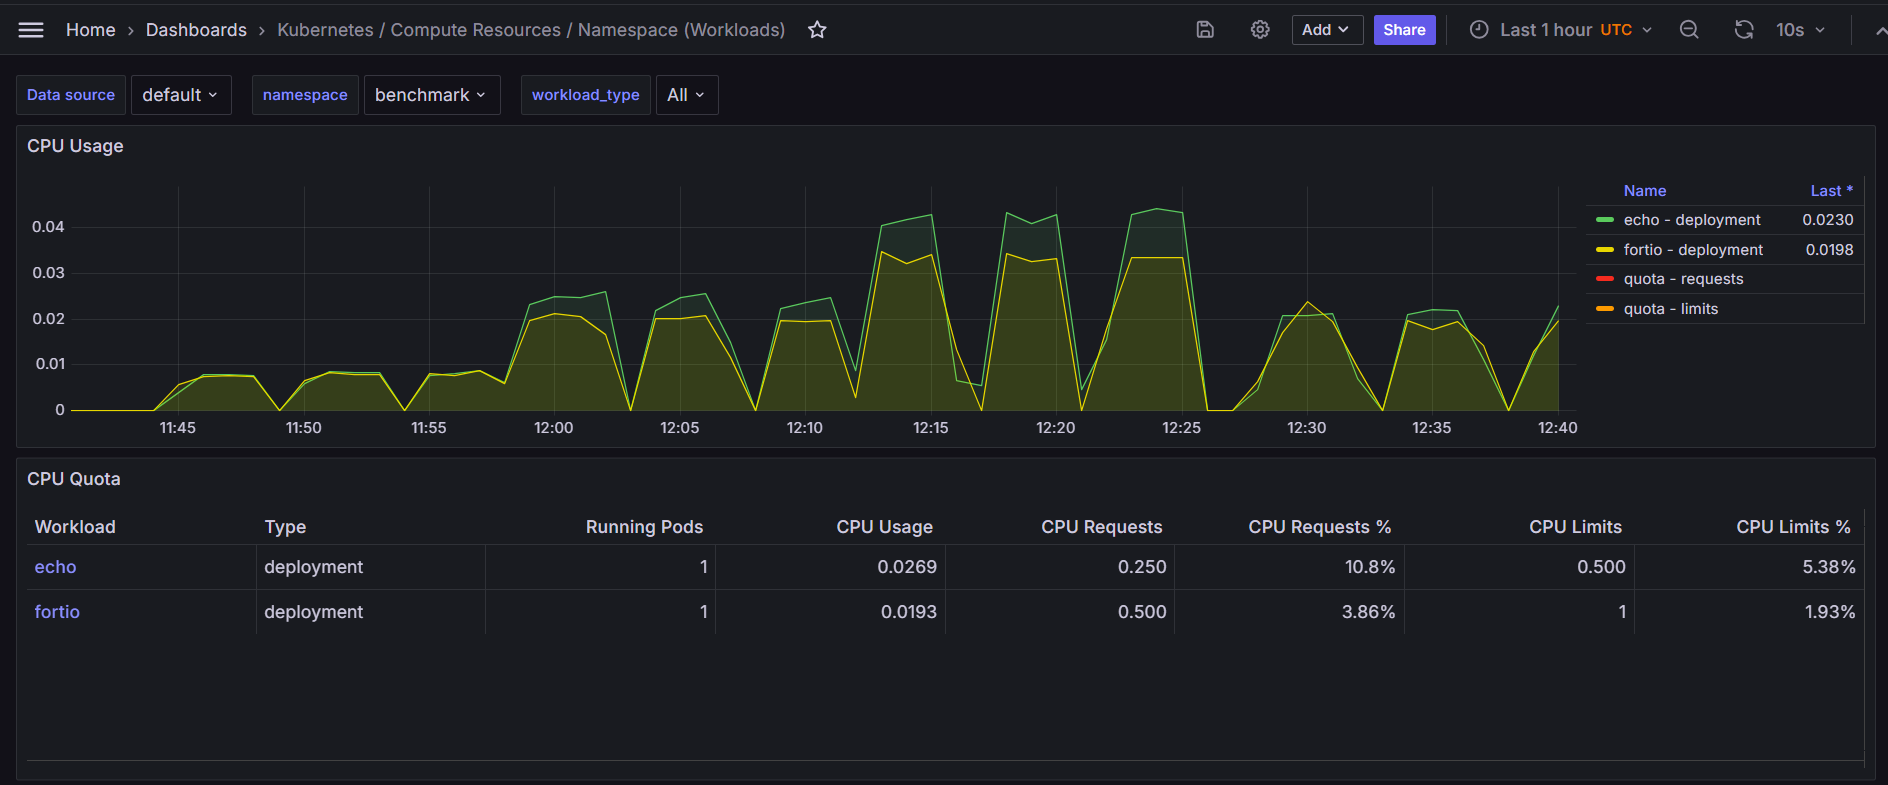
\includegraphics[width=0.92\textwidth]{../figures/grafana/modeB/grafana-ns-cpu-S2-L2.png}
    \caption{Grafana bổ sung cho S2 L2 Mode B: CPU namespace}
    \label{fig:app-s2-l2-modeb-cpu}
\end{figure}

\begin{figure}[H]
    \centering
    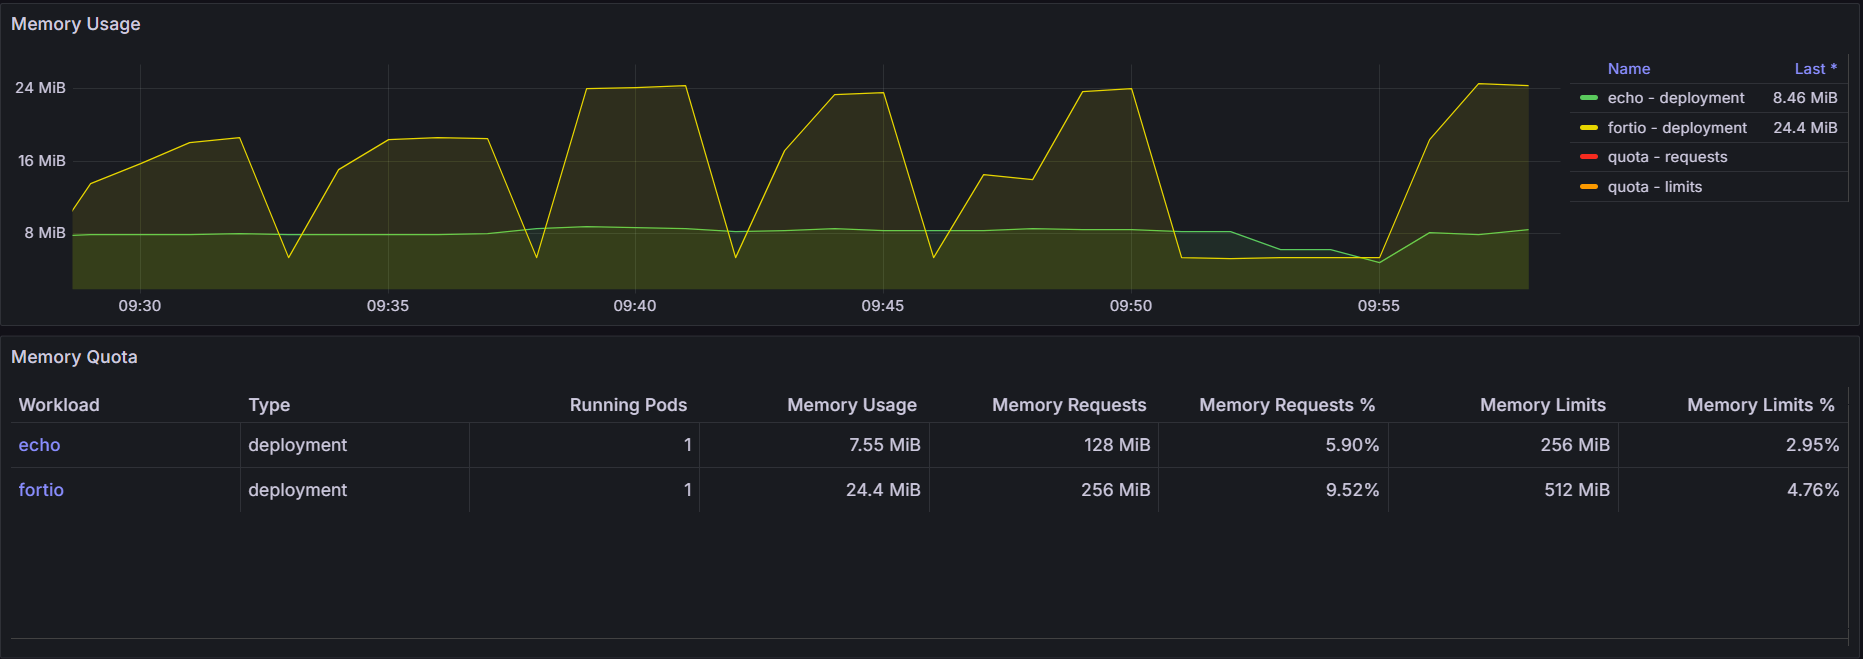
\includegraphics[width=0.92\textwidth]{../figures/grafana/modeA/grafana-ns-mem-S2-L2-R1.png}
    \caption{Grafana bổ sung cho S2 L2 Mode A: memory namespace}
    \label{fig:app-s2-l2-modea-memory}
\end{figure}

\begin{figure}[H]
    \centering
    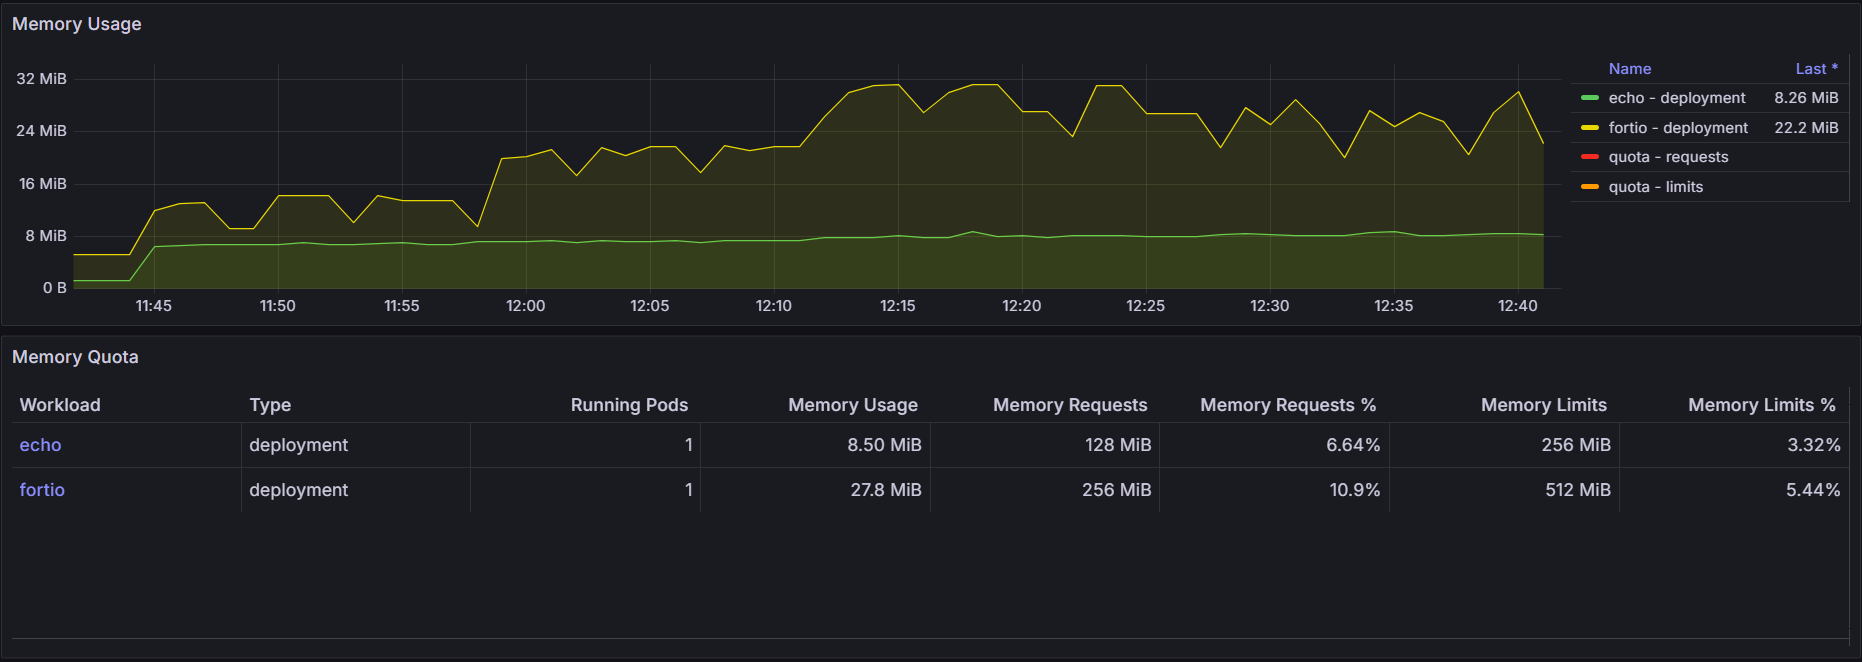
\includegraphics[width=0.92\textwidth]{../figures/grafana/modeB/grafana-ns-mem-S2-L2.png}
    \caption{Grafana bổ sung cho S2 L2 Mode B: memory namespace}
    \label{fig:app-s2-l2-modeb-memory}
\end{figure}

\section{Ảnh Grafana bổ sung cho S3}

S3 là kịch bản so sánh policy OFF/ON trong Mode B, không phải so sánh Mode A với Mode B. Các ảnh dưới đây hỗ trợ kiểm tra bối cảnh vận hành khi policy thay đổi. Chúng không được dùng để kết luận overhead bằng 0; kết luận ở Chương 4 vẫn dựa trên p99, RPS và error rate.

\begin{figure}[H]
    \centering
    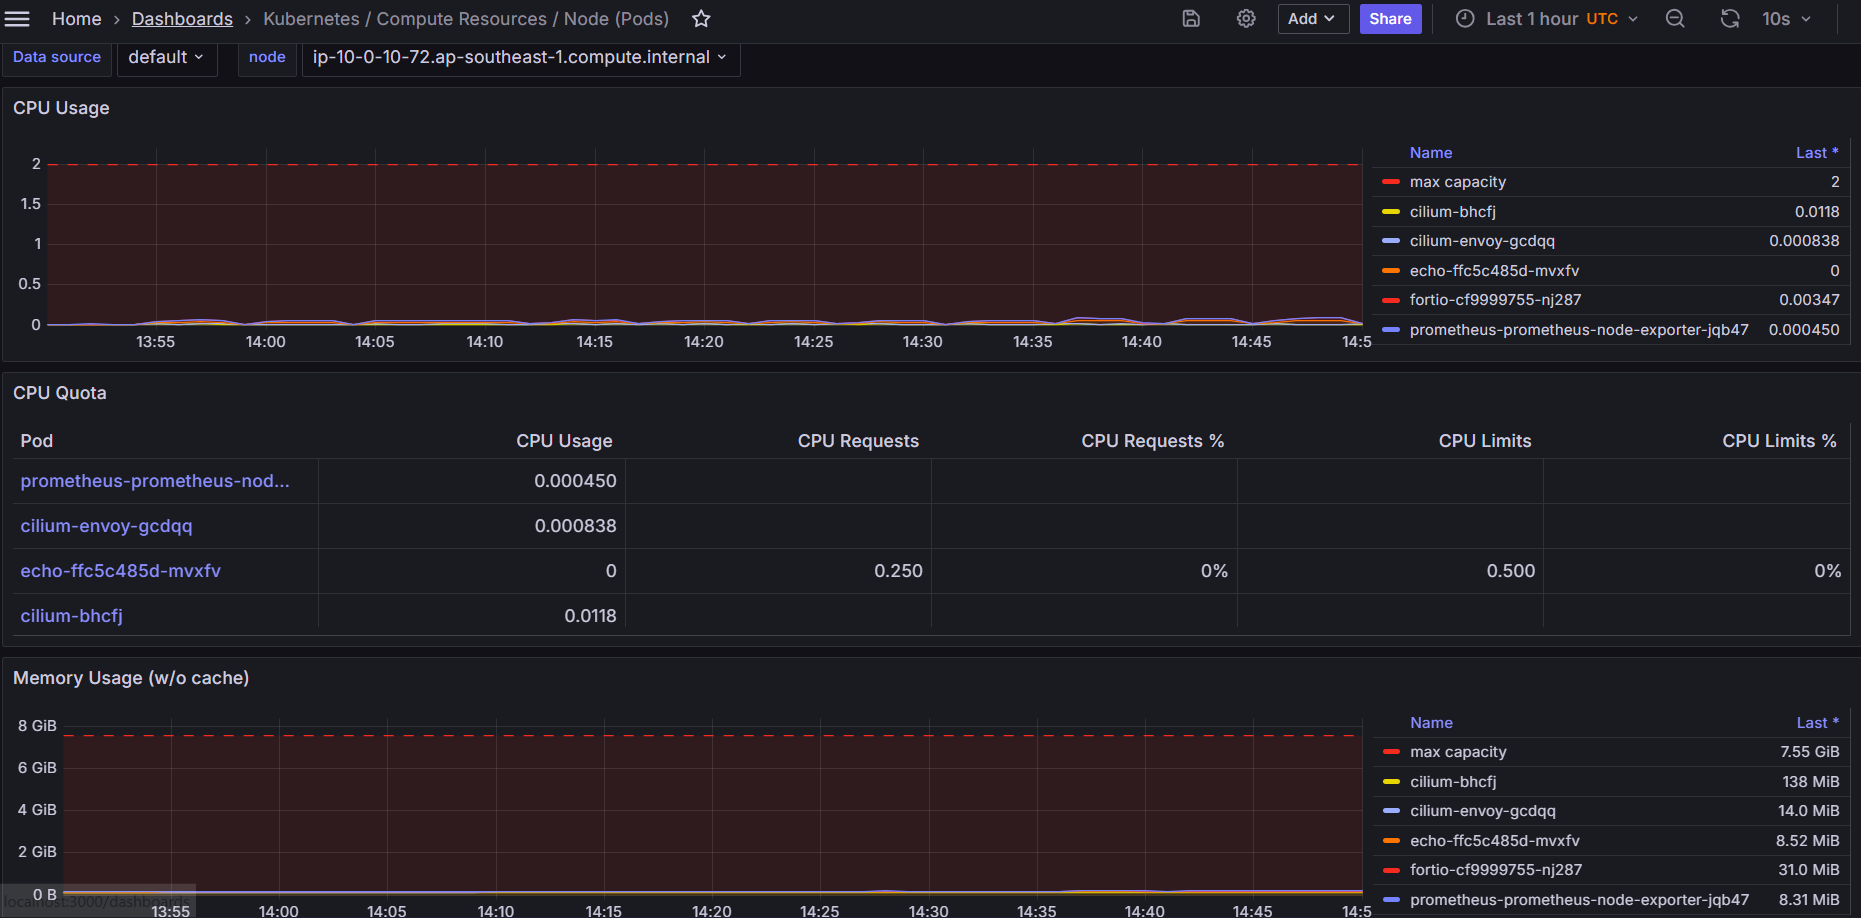
\includegraphics[width=0.92\textwidth]{../figures/grafana/modeB/grafana-ns-node-S3-off-L3.png}
    \caption{Grafana bổ sung cho S3 L3 trong Mode B: policy OFF}
    \label{fig:app-s3-l3-off-node}
\end{figure}

\begin{figure}[H]
    \centering
    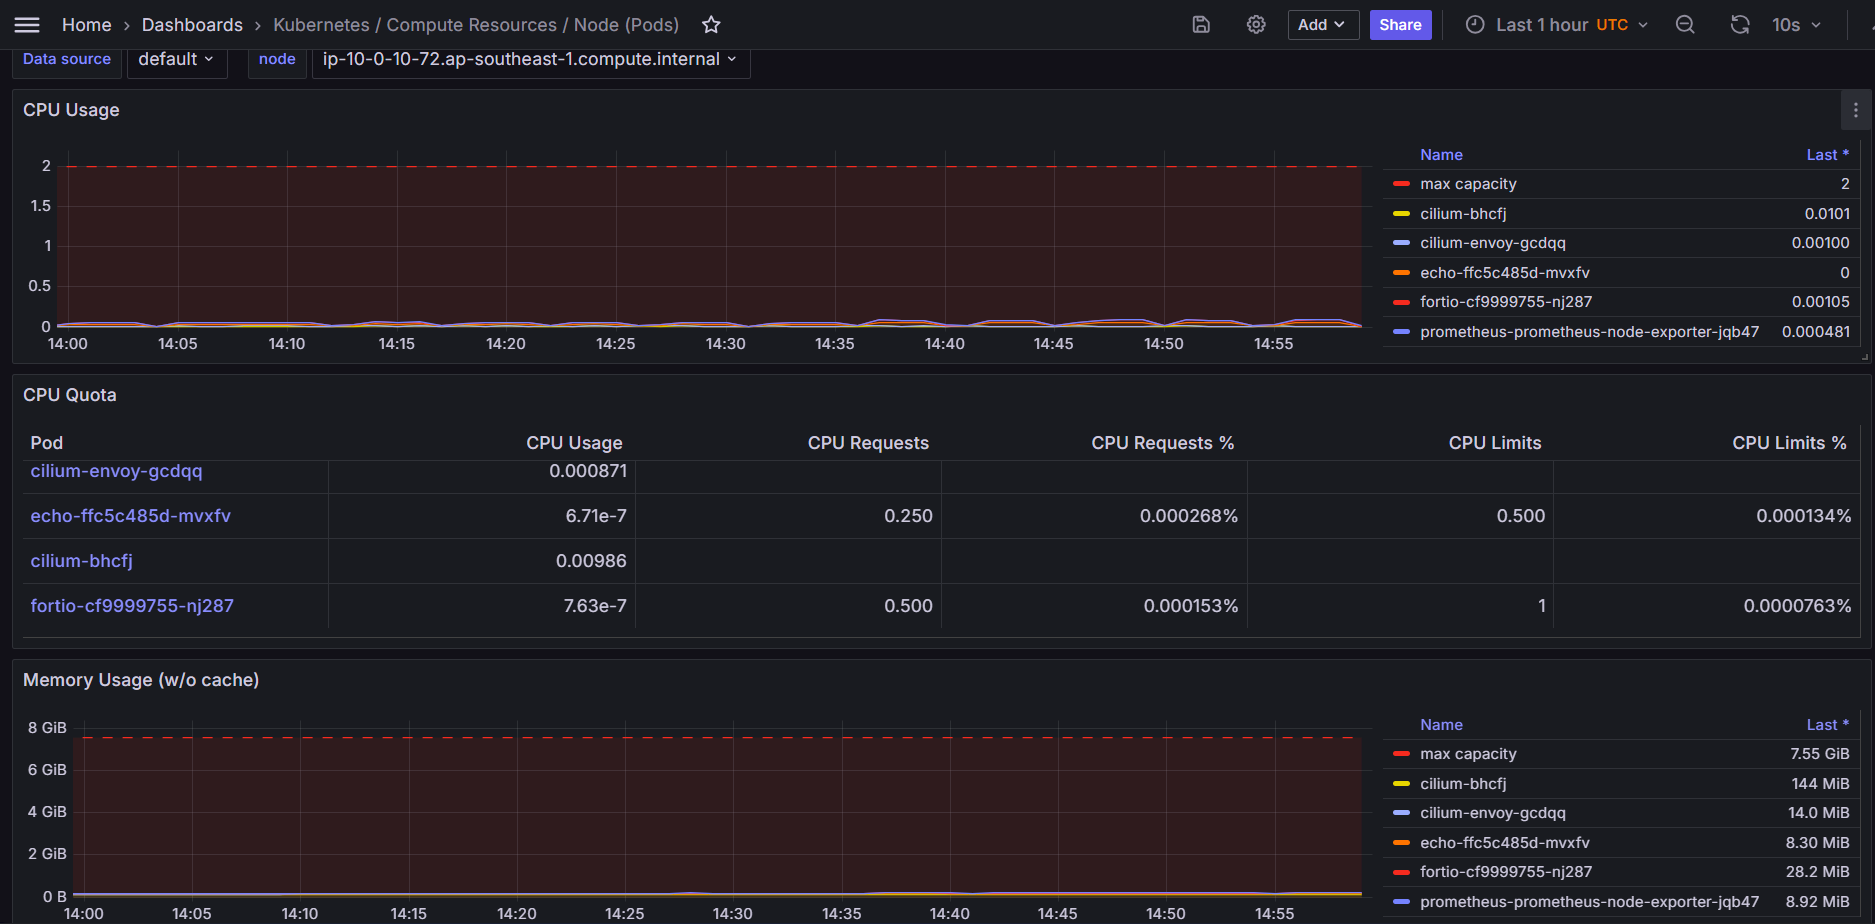
\includegraphics[width=0.92\textwidth]{../figures/grafana/modeB/grafana-ns-node-S3-on-L3.png}
    \caption{Grafana bổ sung cho S3 L3 trong Mode B: policy ON}
    \label{fig:app-s3-l3-on-node}
\end{figure}

\begin{figure}[H]
    \centering
    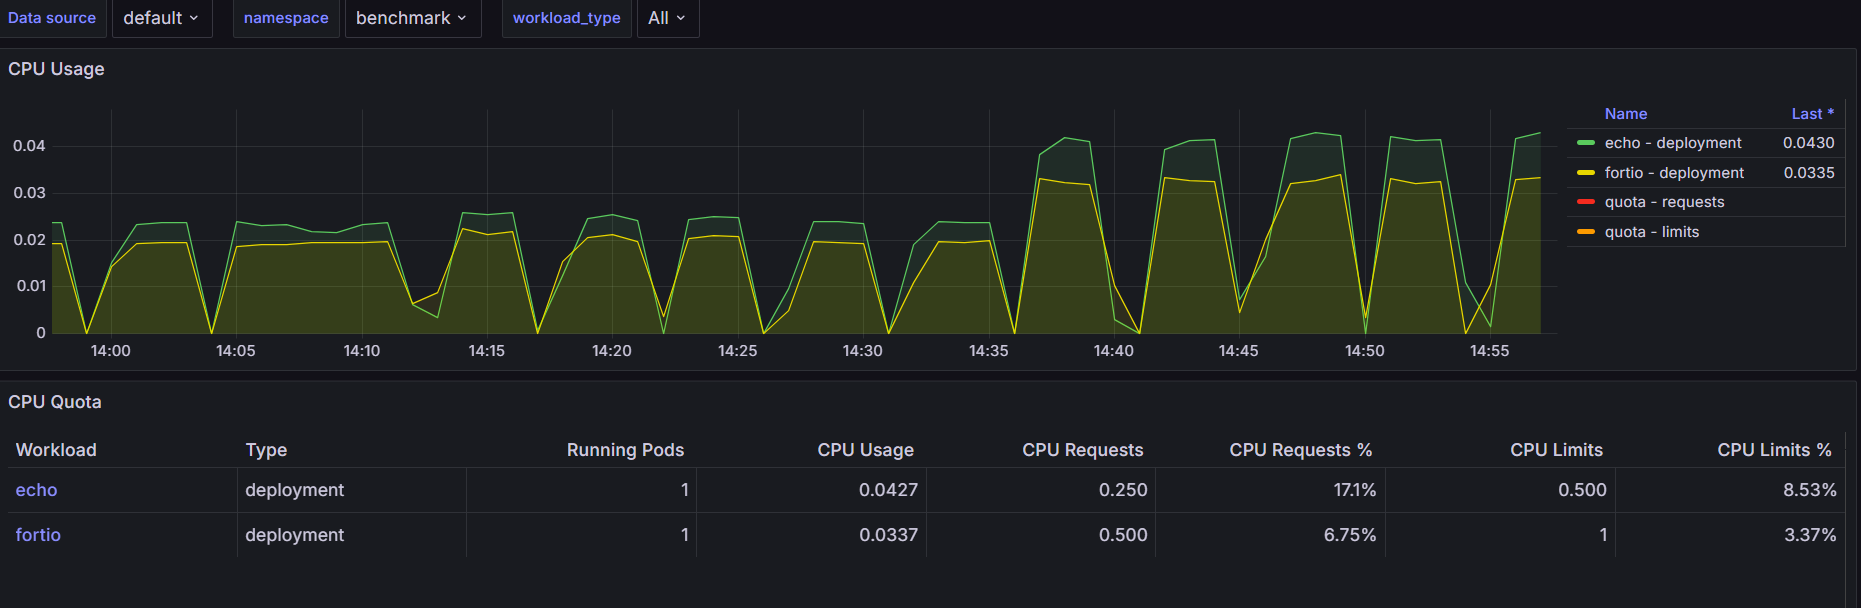
\includegraphics[width=0.92\textwidth]{../figures/grafana/modeB/grafana-ns-cpu-S3-on-L3.png}
    \caption{Grafana bổ sung cho S3 L3 policy ON: CPU namespace}
    \label{fig:app-s3-l3-on-cpu}
\end{figure}

\begin{figure}[H]
    \centering
    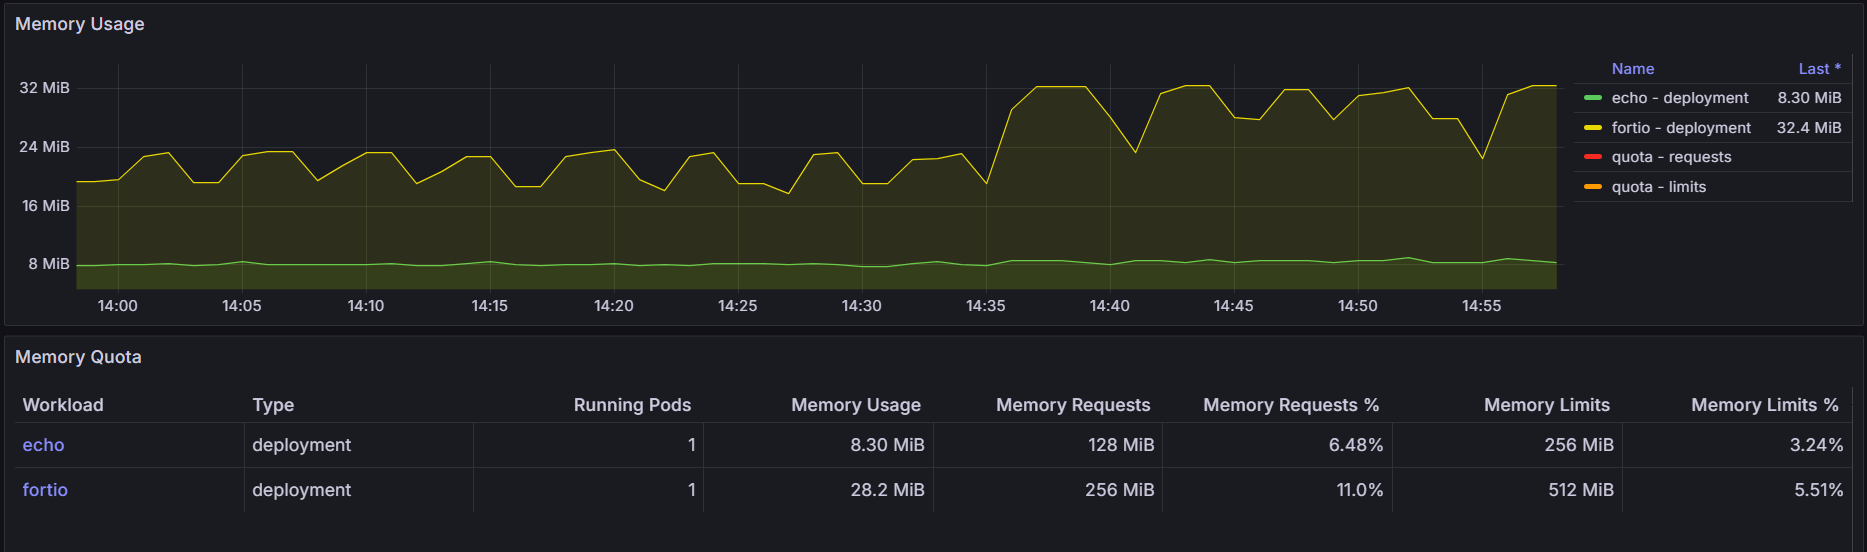
\includegraphics[width=0.92\textwidth]{../figures/grafana/modeB/grafana-ns-mem-S3-on-L3.png}
    \caption{Grafana bổ sung cho S3 L3 policy ON: memory namespace}
    \label{fig:app-s3-l3-on-memory}
\end{figure}

\section{Ảnh Hubble bổ sung}

Các ảnh Hubble dưới đây giúp minh họa thêm trạng thái Hubble, pod kiểm thử deny-case và màn hình chi tiết flow. Các ảnh này chỉ là evidence observability ở mức flow/verdict, không phải packet capture và không phải nguồn đo hiệu năng.

\begin{figure}[H]
    \centering
    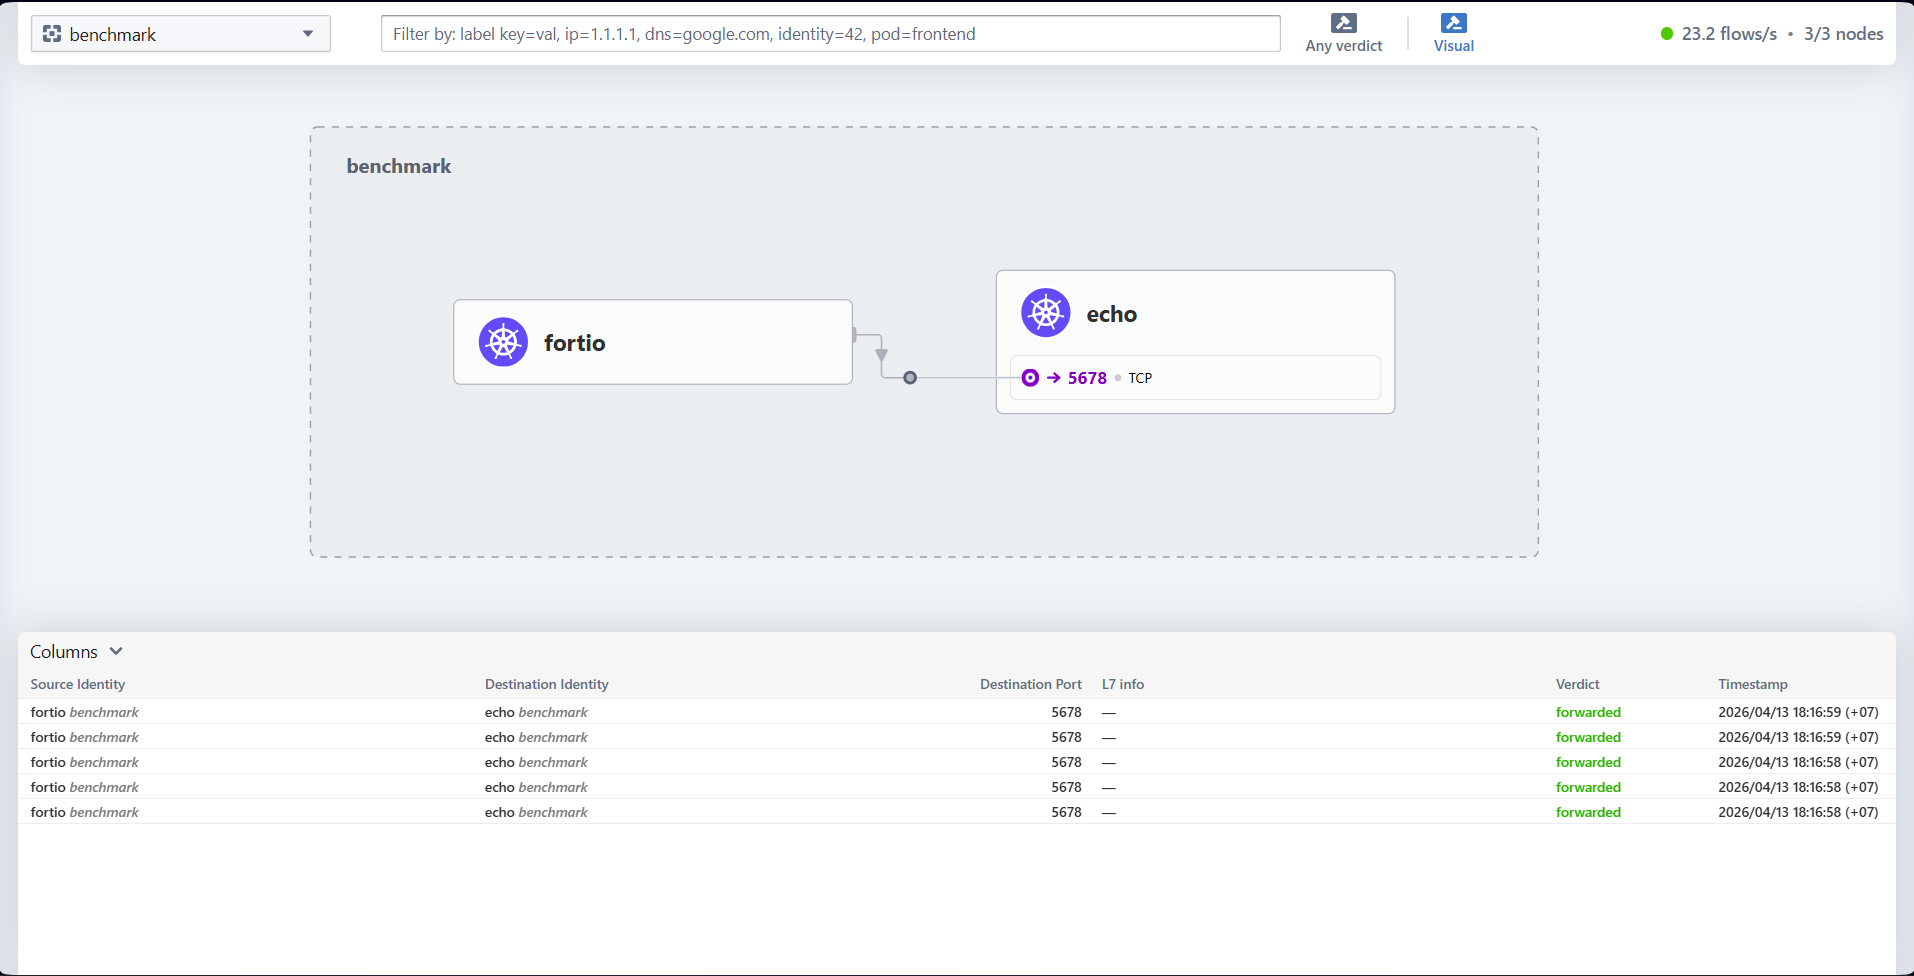
\includegraphics[width=0.92\textwidth]{../figures/hubble/fig-12-modeB-hubble-status.png}
    \caption{Ảnh Hubble bổ sung: trạng thái/flow Hubble trong Mode B}
    \label{fig:app-hubble-status}
\end{figure}

\begin{figure}[H]
    \centering
    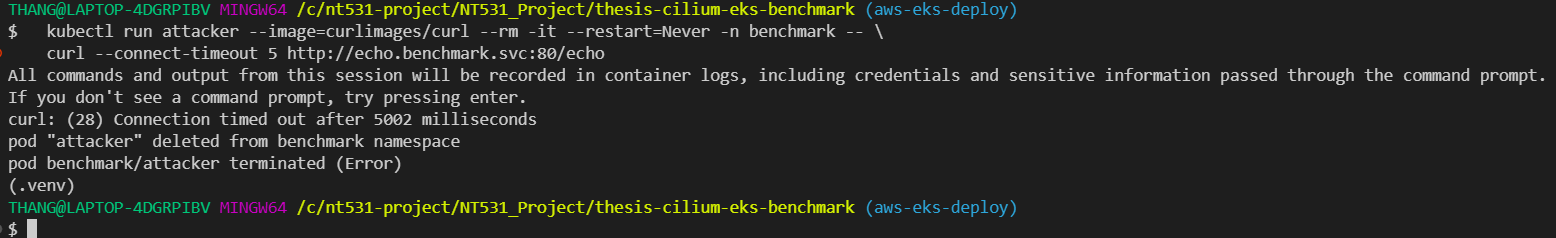
\includegraphics[width=0.92\textwidth]{../figures/hubble/fig-13-hubble-attacker-pod.png}
    \caption{Ảnh Hubble bổ sung: pod dùng cho manual deny-case}
    \label{fig:app-hubble-attacker-pod}
\end{figure}

\begin{figure}[H]
    \centering
    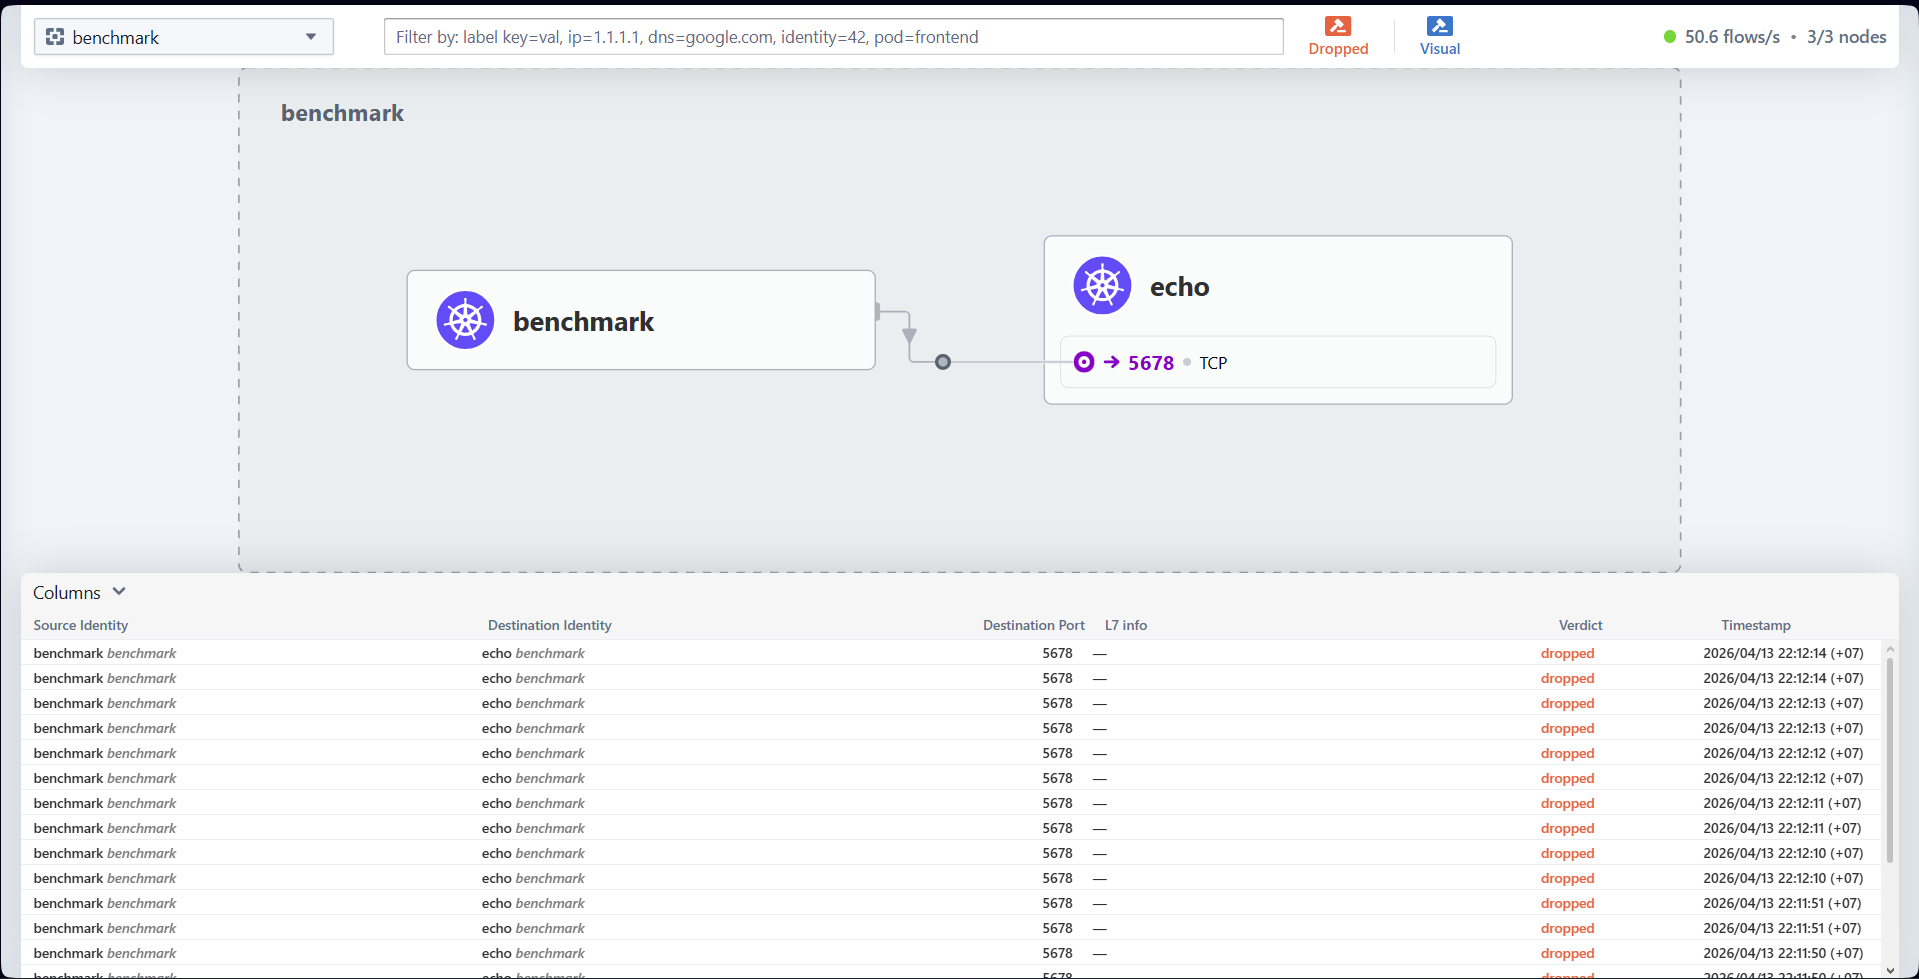
\includegraphics[width=0.92\textwidth]{../figures/hubble/fig-13-hubble-deny-case.png}
    \caption{Ảnh Hubble bổ sung: deny-case ở mức overview}
    \label{fig:app-hubble-deny-overview}
\end{figure}

\begin{figure}[H]
    \centering
    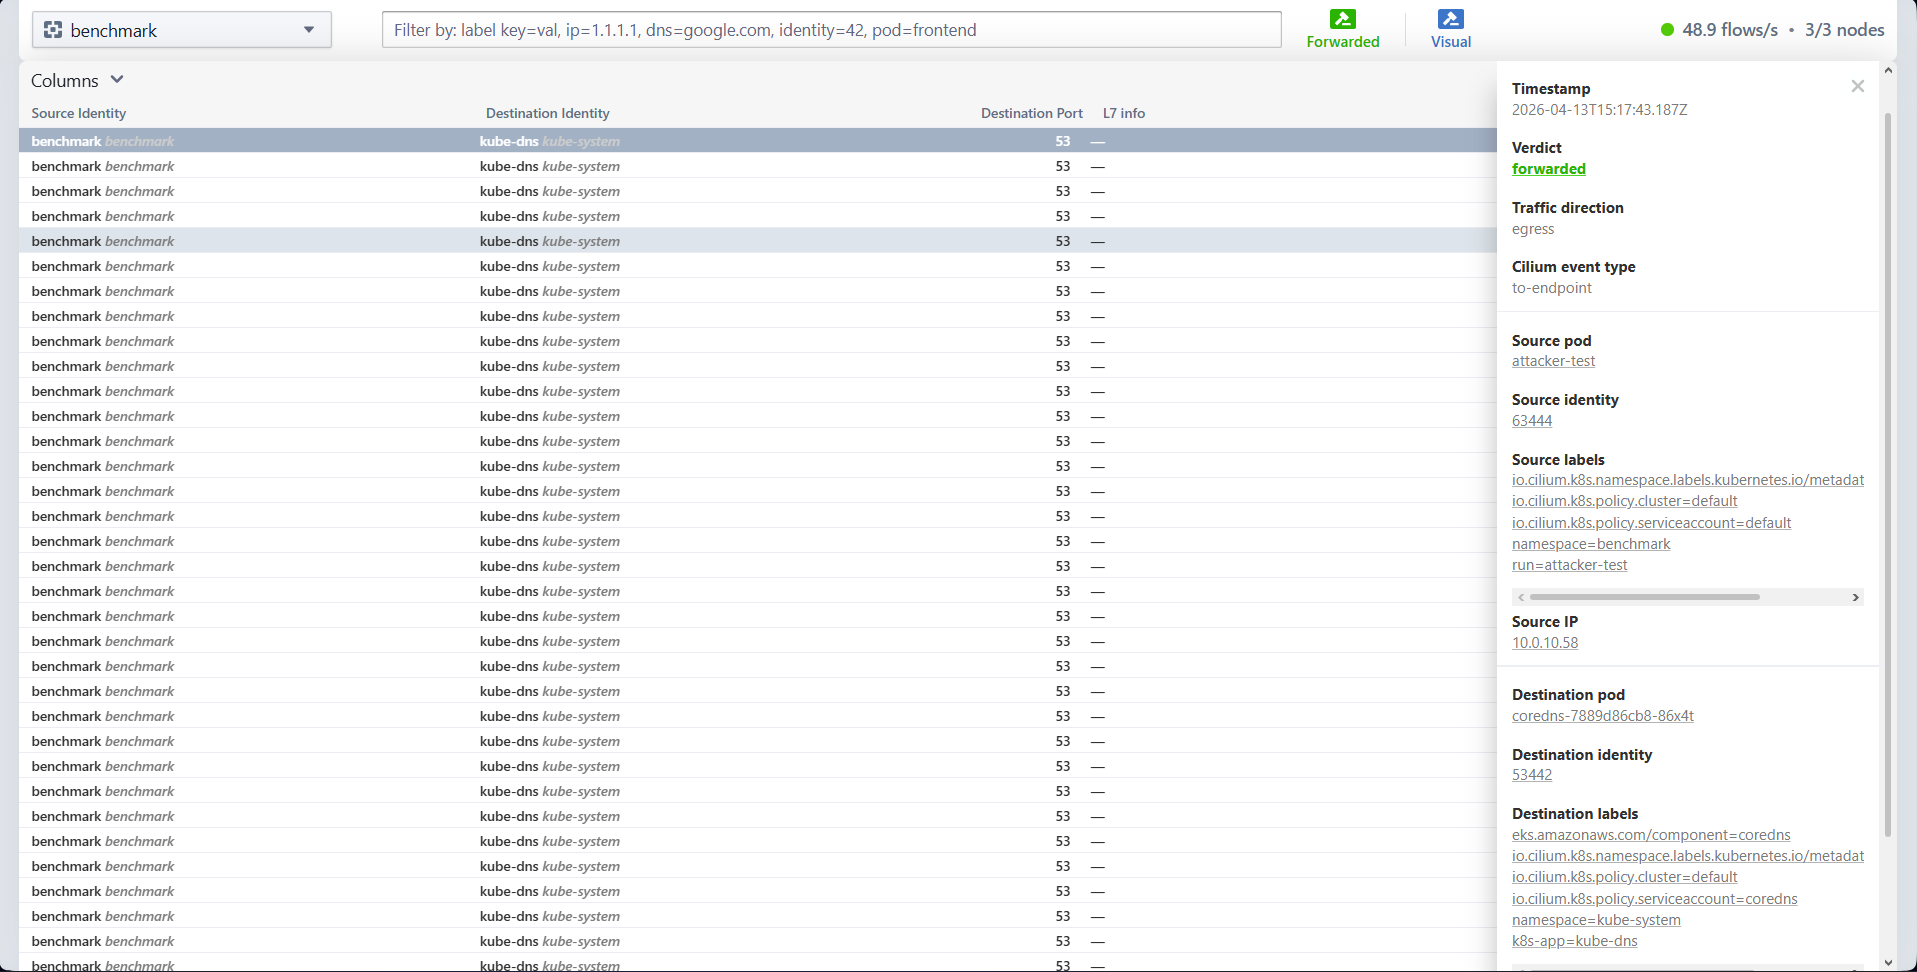
\includegraphics[width=0.92\textwidth]{../figures/hubble/fig-13b-hubble-forwarded-case-detail.png}
    \caption{Ảnh Hubble bổ sung: chi tiết một forwarded flow}
    \label{fig:app-hubble-forwarded-detail}
\end{figure}
